% INTRODUCTION
%

%
%\part{Introduction}
\chapter{Introduction}
\label{chap:intro}

%\cleanchapterquote{You can’t do better design with a computer, but you can speed up your work enormously.}{Wim Crouwel}{(Graphic designer and typographer)}

%In the field of second-language education, pronunciation has traditionally been given less attention than other areas such as grammar or vocabulary \citep{Derwing2005}. One reason for this may be that pronunciation is best taught through one-on-one instruction, which is not often possible in the traditional classroom setting. Hence the attraction of Computer-Assisted Pronunciation Training (CAPT) systems, which have the potential to automatically provide highly individualized analysis of learner errors, and feedback on how to correct them and achieve more intelligible 
%and native-like 
%pronunciation in the target language \citep{Witt2012}. 

%Something about how there's not much CAPT for German?

For students with French as their first language (L1) who are learning German as a second language (L2), the sound system of the L2 can pose a variety of difficulties, one of the most important and interesting of which is the way in which certain syllables in German words are accentuated more than others, a phenomenon referred to as lexical stress. Learning to navigate German lexical stress is especially challenging for L1 French speakers, because this phenomenon is realized very differently (perhaps not at all) in the French language. 

Computer-Assisted Pronunciation Training (CAPT) systems
%, which 
have the potential to automatically provide highly individualized analysis of such learner errors, as well as feedback on how to correct them, and thus to help learners achieve more intelligible 
%and native-like 
pronunciation in the target language \citep{Witt2012}. 
%
The thesis project described here aims to advance 
%the state of the art of 
German CAPT %TODO too intense? reword
by creating a tool which will diagnose and offer feedback on lexical stress errors in the L2 German speech of L1 French speakers, in the hopes of ultimately helping these learners 
%become more sensitive to the lexical stress patterns of German and develop the ability to accurately realize these patterns in their speech. 
become more intelligible when speaking German.



\section{Objectives}
\label{sec:intro:objectives}

%		\begin{floatingfigure}[r]{.5\textwidth}
%			\centering
%			\vspace{-2em}
%			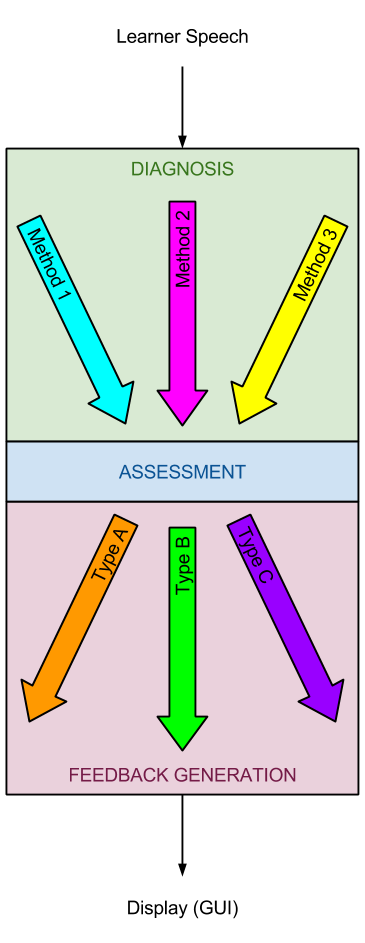
\includegraphics[width=.35\textwidth]{img/hourglass}
%			\vspace{1em}
%			\caption{Conceptual diagram of the prototype CAPT tool.}
%			\label{fig:hourglass}
%			%\vspace{1em}
%		\end{floatingfigure}

The main objective of this work is to investigate the automatic treatment of lexical stress errors in the context of a CAPT system for French learners of German. This includes, on the one hand, an examination of the ways in which lexical stress errors 
	made by these learners
	%of the type made by French L1 speakers when speaking German as L2 
	can be reliably detected %and measured
automatically, and on the other, an exploration of the types of multimodal feedback 
	%on such errors 
	that can be automatically delivered based on this error detection. 
%
%
%The outcome of these investigations is a prototype CAPT tool, conceptually illustrated in \cref{fig:hourglass-ITS},
%which can diagnose lexical stress errors in different ways and present learners with different types of feedback on these errors. 
%
The outcome of these investigations and primary contribution of this thesis project is a prototype CAPT tool called 
%
%\TODO{pick one:}
%
%\textit{de-stress}: the German (\underline{de}) \underline{S}ystem for \underline{T}raining and \underline{R}esearch on \underline{E}rrors in \underline{S}econd-language \underline{S}tress. 
%
\textbf{de-stress}: the German (\textbf{de}) \textbf{S}ystem for \textbf{T}raining and \textbf{R}esearch on \textbf{E}rrors in \textbf{S}econd-language \textbf{S}tress. 
%
Implemented as a web application in the Java-based language Groovy\footnote{\url{http://groovy-lang.org}} using the Grails web framework,\footnote{\url{https://grails.org}} de-stress is open-source and publicly available online.\footnote{\url{https://github.com/vakila/de-stress}}
\Cref{fig:hourglass-ITS} provides a conceptual overview of the tool, which provides a variety of options for diagnosis of and feedback on lexical stress errors, and could potentially be a useful component of a fully-fledged intelligent CAPT system (a type of Intelligent Tutoring System, or ITS). 

	\begin{figure}[tb] 
		\centering
		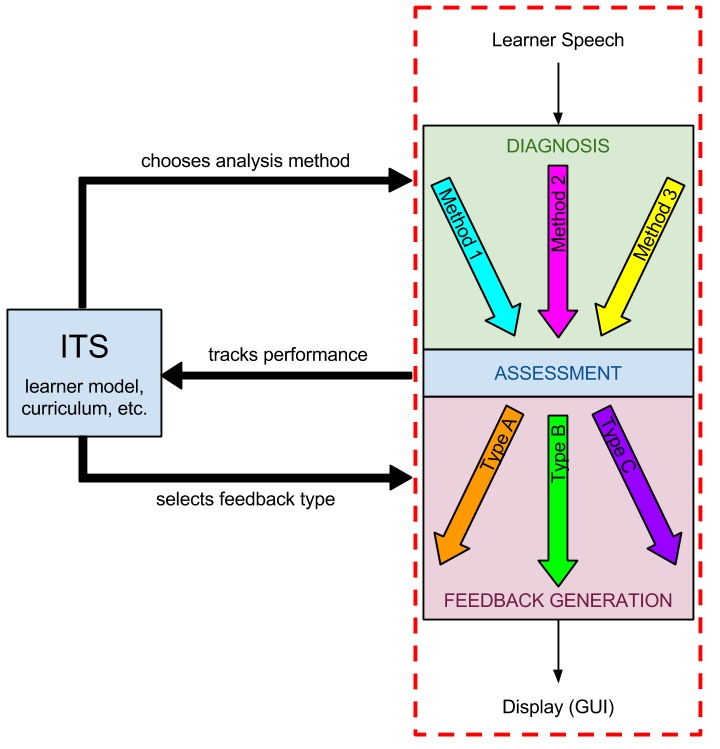
\includegraphics[height=.45\textheight]{img/hourglass-ITS} 
		\caption[Conceptual diagram of the prototype lexical stress CAPT tool]{Conceptual diagram of the prototype lexical stress CAPT tool (demarcated by dashed line) and its possible function in the context of a more comprehensive Intelligent Tutoring System (ITS).}
		\label{fig:hourglass-ITS}
	\end{figure}

 Via a simple web interface, the system presents a student with a German sentence,
 %(taken from the IFCASL corpus), 
 one of the words of which is highlighted as the target word for that exercise. The student is prompted to submit an utterance of that sentence for assessment and feedback, with the instruction to focus on the accurate expression of the lexical stress pattern of the target word. The student's utterance is subsequently analyzed for lexical stress errors using a variety of diagnostic approaches (see \cref{chap:diagnosis}), and finally the student is presented with one or more types of feedback on their realization of lexical stress in the analyzed utterance (see \cref{chap:feedback}). \Cref{fig:interface:student} presents a screenshot of the interface presenting such feedback.

	\begin{figure}[htb]
		\centering
		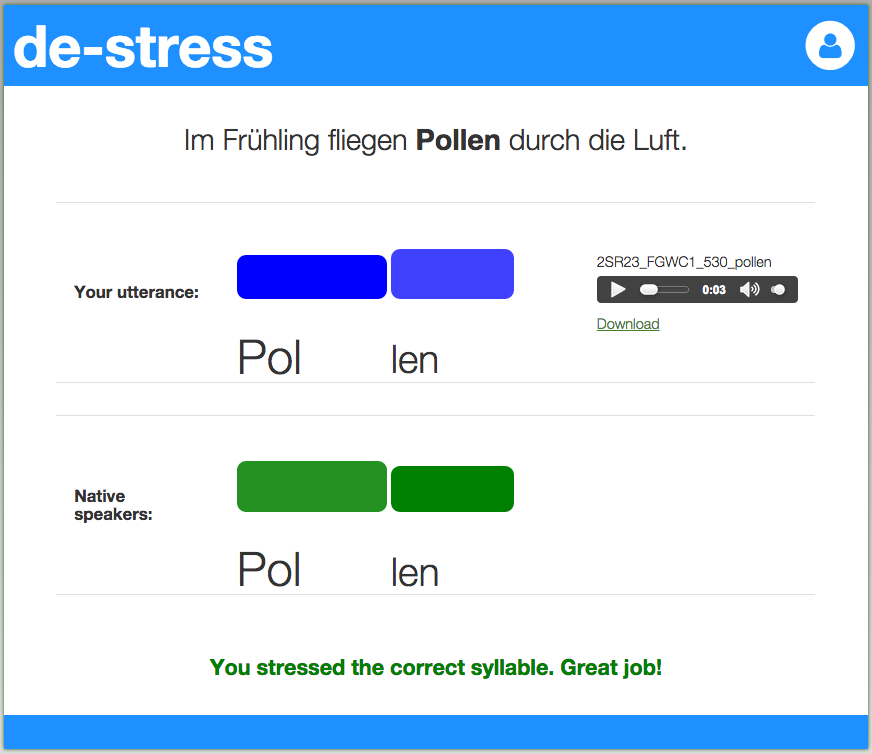
\includegraphics[width=\textwidth]{img/screenshots/StudentInterface-userIcon}
		\caption{The student-facing interface of de-stress}
		\label{fig:interface:student}
	\end{figure}

In addition to this student-facing interface, 
%the tool also implements an interface through which 
an administrative interface allows
a language teacher or a researcher of L2 language acquisition 
%can 
to
create new exercises for students to complete, where each exercise features a specific combination of the various diagnostic methods and feedback types available in the system. By allowing fine-grained control over these features, de-stress enables researchers to create CAPT exercises with different features for the purposes of in vivo studies of the effectiveness of different feedback types, and allows teachers to create exercises matching the needs of their students. The 
%teacher- or researcher-facing
administrative interface for exercise creation can be seen in \cref{fig:interface:teacher}.

	\begin{figure}[htbp]
		\centering
		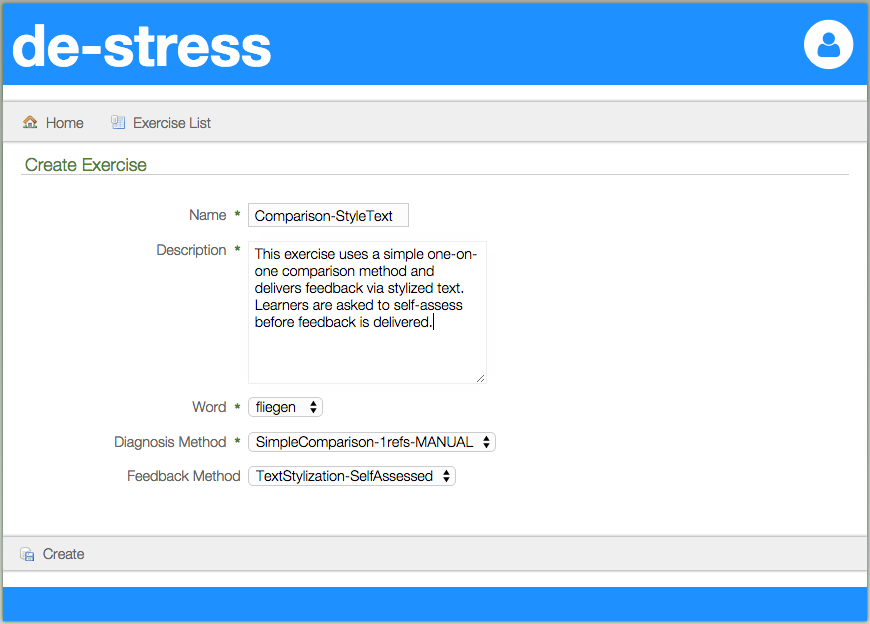
\includegraphics[width=\textwidth]{img/screenshots/TeacherInterface-userIcon}
		\caption{The interface of de-stress for teachers/researchers}
		\label{fig:interface:teacher}
	\end{figure}

%\TODO{This prototype tool} has thus been developed with both instructional and research applications in mind.
Both instructional and research applications have thus motivated the development of de-stress.
Unlike with some existing tools for diagnosis and feedback on pronunciation errors, learners can interact with the tool and interpret its feedback independently, i.e. without the assistance of a human instructor at their side.
At the same time, researchers can use this modular system to study the impact of various assessment and feedback types on learner outcomes, user engagement, and other factors impacting the success of a CAPT system. 
%
Once more is known about which diagnosis/feedback types should be delivered to which learners in which situations, this tool could become a useful component of a fully-fledged intelligent CAPT system, in which 
%learner models and other intelligent components
models of relevant aspects of the learning context (e.g. the student's skill level, progress, or personal preferences; the current learning objective or position in a sequence of exercises; etc.)
are used to automatically decide which modules of the tool to activate, as \cref{fig:hourglass-ITS} illustrates.




\section{Context: The IFCASL project}
\label{sec:intro:ifcasl}

This work has been conducted in the context of the ongoing 
%Franco-German 
research project ``Individualized Feedback in Computer-Assisted Spoken Language Learning'' (IFCASL)\footnote{\url{http://www.ifcasl.org}}
The project brings together researchers 
 at 
{\thesisUniversity} 
%Saarland University 
 (Saarbrücken, Germany) and LORIA (Nancy, France), and 
is supported by the Deutsche Forschungsgemeinschaft (DFG) and the Agence Nationale de la Recherche (ANR).

The goal of the IFCASL project is to take initial steps toward the development of a CAPT system targeting
%, on the one hand, 
native (L1) French speakers learning German as a foreign language (L2), 
as well as
%and on the other, 
L1 German speakers learning French as their L2. To this end, one of the major project objectives has been the compilation of a bidirectional learner speech corpus for the French-German language pair. Comprising phonetically diverse utterances in French and German spoken by both native speakers and nonnative speakers with the other language as L1 \citep{Fauth2014,Trouvain2013}, this is the first known corpus of L2 speech in both directions of this language pair.

As described by \textcite{Trouvain2013,Fauth2014}, the IFCASL corpus contains recordings of approximately 100 speakers (50 native speakers of each of the two languages) uttering carefully constructed stimuli in both languages, such that speech in both the L1 and L2 was recorded for each speaker. In recording sessions, subjects were asked to read aloud a given sentence or longer text, and for approximately half of the L2 stimuli, subjects were allowed to listen to a recording of the text as uttered by a native speaker 
%of the target language 
before recording their utterance. An even gender distribution was maintained among the speakers recorded, and both children (adolescents under 18 years of age) and adults participated in the recordings, the majority of participants being adults. While children were uniformly of beginner proficiency in their L2, adults of both beginner and advanced levels in the L2 were recorded. Additional details about the corpus and its participants are given in \cref{sec:lexstress:data}.


The German-language subset of the IFCASL corpus has been instrumental in training and testing the automatic diagnosis and feedback systems developed in this work.
 (While the IFCASL project as a whole is also concerned with L1 German speakers learning French as L2, and the 
 collected recordings are
 %corpus collected in the project is 
 evenly distributed between the two languages, this thesis focuses exclusively on French L1 speakers learning German as L2.) 
 %
As the IFCASL corpus had not been annotated for lexical stress errors, one major contribution of this thesis project is 
the collection of error annotations 
%the annotation of such errors 
for a subset of the German-language utterances by L1 French speakers; the details of this annotation effort are described in \cref{chap:lexstress}. 

Furthermore, 
de-stress
%\TODO{the prototype CAPT tool developed in this thesis project}
 has been designed with a view to contributing to the overall set of software developed in the context of the IFCASL project, such that it is as compatible as possible with the other tools developed and used by the IFCASL team, especially the JSnoori speech processing software developed at LORIA (see \cref{sec:capt:snoori}).




\section{Thesis overview}
\label{sec:intro:overview}


\myemph{\Cref{chap:background}: \nameref{chap:background}} introduces Computer-Assisted Pronunciation Training (CAPT) 
%in the contexts of pronunciation teaching in foreign-language education and computer-based and intelligent tutoring systems, describing 
and describes some relevant past work on CAPT systems. 
This chapter also briefly 
%outlines the differences in the lexical stress systems of French and German as well as 
introduces the phenomenon of lexical stress as it pertains to L1 French learners of German as L2, and outlines
the motivation for focusing on lexical stress errors in this work.


\myemph{\Cref{chap:lexstress}: \nameref{chap:lexstress}} 
%explores lexical stress in the speech systems of French and German in more detail, describing relevant findings from past work on lexical stress and its acoustic correlates in these languages. 
%This chapter also 
describes 
%original work on 
%one of the major contributions of this thesis: 
the annotation and analysis of lexical stress errors in 
%the IFCASL sub-corpus of 
nonnative German speech produced by native French speakers, which constitutes an important contribution of this thesis. 
The annotation process and the resultant findings with respect to the distribution of lexical stress errors in L2 German speech are presented in detail in this chapter.

\myemph{\Cref{chap:diagnosis}: \nameref{chap:diagnosis}} details how de-stress diagnoses lexical stress errors in learner speech. It describes the methods used to automatically segment the learner's utterance, analyze the prosody of this utterance in terms of the relative pitch, duration, and intensity of the relevant syllables, and compare this analysis to one or more models of native pronunciation to produce a diagnosis. The novel diagnostic approaches described in this chapter comprise another major contribution of this work. 
% described in this chapter include novel methods for error diagnosis by comparison with one or more reference utterances

\myemph{\Cref{chap:feedback}: \nameref{chap:feedback}} 
%describes the multimodal feedback options that the system can deliver, and how these feedback types are generated based on the analysis of the learner's speech described in the previous chapter. 
describes the final contribution of this project: the feedback module of de-stress, which is capable of delivering a variety of feedback types simultaneously or in isolation. 
This chapter explains the types of feedback available, and how these are generated from the diagnosis of the learner's speech described in \cref{chap:diagnosis}.

%\myemph{\Cref{chap:system}} briefly introduces the tools that have been developed, and the technology used to build them. \TODO{skip this chapter?}

\myemph{\Cref{chap:conclusion}: \nameref{chap:conclusion}} summarizes the ways in which this thesis project has contributed to the advancement of CAPT for French learners of German,
%This chapter also 
and
outlines some
possible directions for future extensions of this work.




%\section{Proposal overview}
%The remainder of this proposal is structured as follows.
%
%TODO update - this is the old overview from the proposal
%\Cref{chap:background} places this thesis in the context of existing research on CAPT, and motivates its specific focus on lexical stress errors.
%\Cref{chap:diagnosis} outlines the techniques to be explored for diagnosing lexical stress errors in learners' speech via automatic processing of acoustic correlates of these errors in a spoken utterance.
%\Cref{chap:feedback} describes the multimodal feedback types the system will aim to deliver, 
%%and how these could be generated automatically from 
%based on
%the analysis described in the previous section.
%\Cref{sec:conclusion} summarizes the proposal and the aims of the thesis.

